\section{Les classes d'agents}
\subsubsection{Sprints 1 et 2}
Lors du premier sprint, nous avons commencé par mettre en place la base du programme. Nous avions prévu de réaliser l'UML figure~\ref{v0.1}.

 Pour le modèle, il s'agissait de créer les classes :
\begin{itemize}
\item \verb|Turtle|, qui représente une tortue~;
\item \verb|Point|, pour stocker les coordonnées d'une tortue~;
\item \verb|Line|, qui est composé de points, et qui permet aux tortues de laisser une trace (instruction \verb|pen_down|)~;
\item \verb|World|.
\end{itemize}


\begin{figure}[h]
\centering
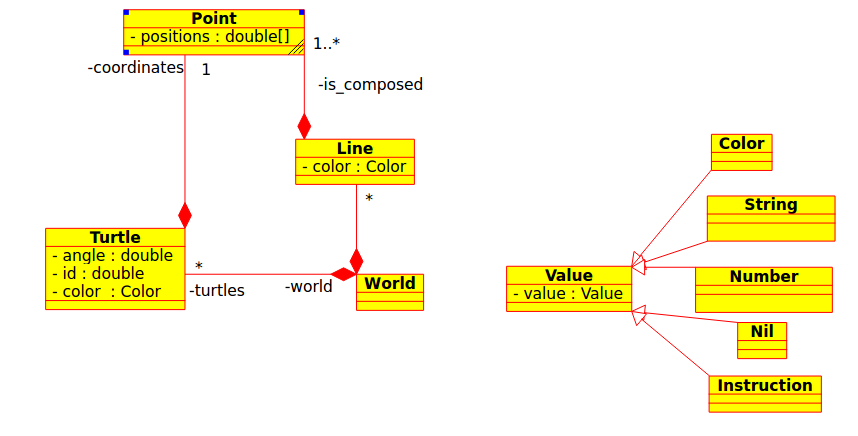
\includegraphics[scale=0.5]{doc/report/uml/v01.png}
\caption{\label{v0.1} UML prévisionnel de la version 0.1}
\end{figure}


La classe \verb|World| représente le monde, contenant la liste des tortues, et les lignes tracées par celles-ci, et communique avec l'interface pour l'affichage.
À la fin du sprint 1, on pouvait voir une tortue avancer et tracer une ligne sur son passage.
Nous avions réalisé le schéma \ref{v0.1R}. Il respecte la version prévue, en dehors de la classe \verb|Instruction|, qui n'était finalement pas nécessaire, les instructions étant des méthodes de \verb|Turtle|.

Lors du second sprint, nous avons ajouté une classe \verb|Agent|, super-classe de \verb|World|, \verb|Turtle| et \verb|Zone|~; en effet, elles sont toutes les trois des agents, et ont donc des comportements similaires (cf. Figure~\ref{v0.2}).

Ces classes contiennent chacunes un parent, une liste d'enfants, et des propriétés. Les propriétés sont des variables définies par l'utilisateur lors de la définition du code de l'agent, donc surtout utile pour les tortues.

De plus, le monde a une taille et deux listes d'espèce de tortues (\verb|Breed|)~: les espèces nommées et les anonymes.

Comme le montre le listing \ref{nameTurtle}, on peut créer des tortues nommées ou pas. Une tortue anonyme a son corps défini à la création de l'agent (lors du \verb|new agent|) tandis que les tortues nommées on leur corps défini lors de la création du type d'agent (instruction \verb|agent <nom>|).

\begin{lstlisting}[language=Stibbons,label=nameTurtle,caption=Nommage lors de la création d'une tortue]
agent listener () {
	fd 2
}

new listener ()

new agent {
	lt 30
	fd 5
}
\end{lstlisting}

\subsubsection{Sprints 3 et 4}
Lors du troisième sprint, nous avons mis en place des pointeurs intelligents dans toutes nos classes (cf. Figure~\ref{v0.3}). Le but de ce sprint était la mise en place de la communication entre les agents~: les tortues devaient pouvoir communiquer via les zones par modification de leurs propriétés, et elles devaient aussi pouvoir communiquer entre elles grâce à des instructions comme \verb|send| et \verb|recv|.

L'étape suivante était d'ajouter des fonctionnalités telles que la maîtrise du temps et l'exportation du modèle. Ces ajouts ne provoquent pas de changements majeurs du côté du modèle, si ce n'est quelques méthodes dans les classes \verb|World|, \verb|Turtle| et \verb|Zone| pour l'export du modèle.
Celui-ci consiste à créer une sauvegarde de l'état du modèle à un instant \verb|t| dans un fichier JSON grâce à la bibliothèque JSON Spirit (cf. Listing \ref{json} ).
Cela permettra ensuite, par exemple en passant par une transformation en CSV, d'avoir des tableaux avec toutes les données, ce qui offre la possibilité d'avoir des diagrammes de l'évolution du monde.

La maîtrise du temps se fait grâce à un bouton pause, qui arrête les threads s'exécutant, ou par un slider qui permet de ralentir ou de diminuer la vitesse.

\section{Les types}
\subsubsection{Sprints 1 et 2}
Lors du premier sprint, nous avons mis en place un certains nombre de types (cf. Figure~\ref{v0.1R}), comme \verb|Color|, représentant les couleurs, ou encore \verb|Nil|, représentant la valeur nulle. Ils héritent de \verb|Value|, une classe abstraite qui contient une valeur et ses accesseurs.

\begin{figure}[h]
\centering
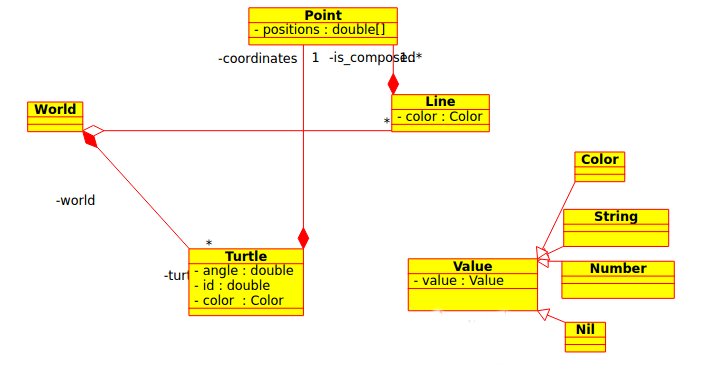
\includegraphics[scale=0.5]{doc/report/uml/v01reel.png}
\caption{\label{v0.1R} UML de la version 0.1 réalisée}
\end{figure}

Lors du second sprint, les types Stibbons sont les mêmes mais leurs définitions se sont un peu complexifiées, en passant par une classe \verb|SimpleValue| pour la mise en place des mutex. Une énumeration des types Stibbons existe, elle est utilisée avec la méthode \verb|getType()| pour pouvoir connaître le type d'une valeur.
Pour que l'utilisateur puisse écrire des fonctions dans le code, nous avons ajouté une classe \verb|Function|, qui stocke un arbre abstrait, contenant le code de la fonction déjà analysé.
Des mutex ont également été ajoutés dans toutes les classes pour assurer que les objets soient thread-safe (cf.~\ref{v0.2}).

\begin{figure}[h]
\centering
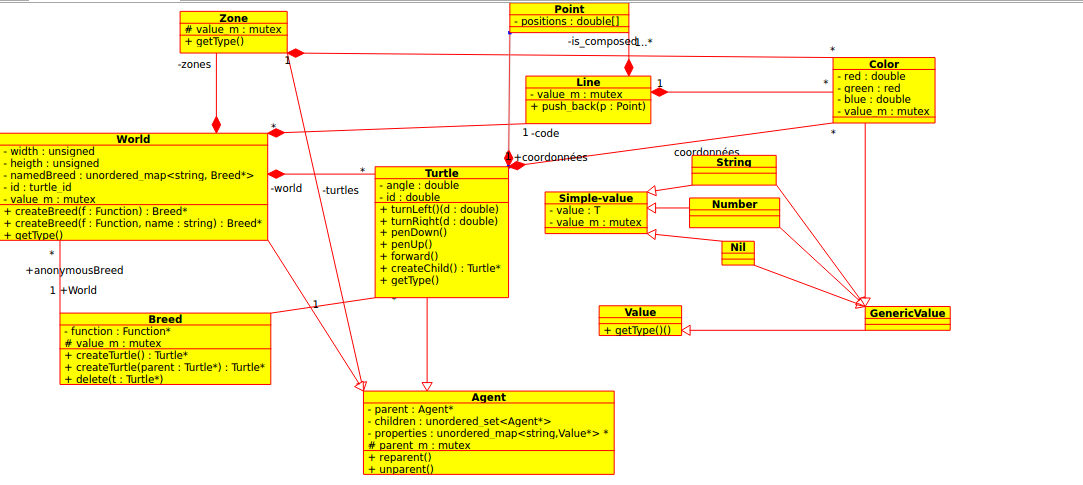
\includegraphics[scale=0.45]{doc/report/uml/v02.png}
\caption{\label{v0.2} UML version 0.2}
\end{figure}

\subsubsection{Sprints 3 et 4}
Lors du troisième sprint, nous avons ajouté une sous-classe de \verb|Function|, \verb|userFunction|, qui représente les fonctions créées par l'utilisateur (cf. Figure~\ref{v0.3}). Nous avons également créé des fonctions standard comme \verb|ask_zone|, qui permettent de donner des ordres aux zones.

L'ajout de \verb|Table| représentant l'unique type de conteneurs, les tableaux, fait aussi parti de ce sprint.
Nous les écrivons à la façon de PHP (cf. Listing~\ref{tablephp}).
\begin{lstlisting}[label=tablephp,caption=Syntaxe des tables en Stibbons]
a = 12

t = {18,red,"bla"}
v = { "bla" : "blou", "blue" : blue, a : 29 }

println(t[2])
t[2] = 32
println(t[2])
v[] = 48
println(v)

u = 5 new agent {
	while true fd 20
}
\end{lstlisting}

\begin{figure}[h]
\centering
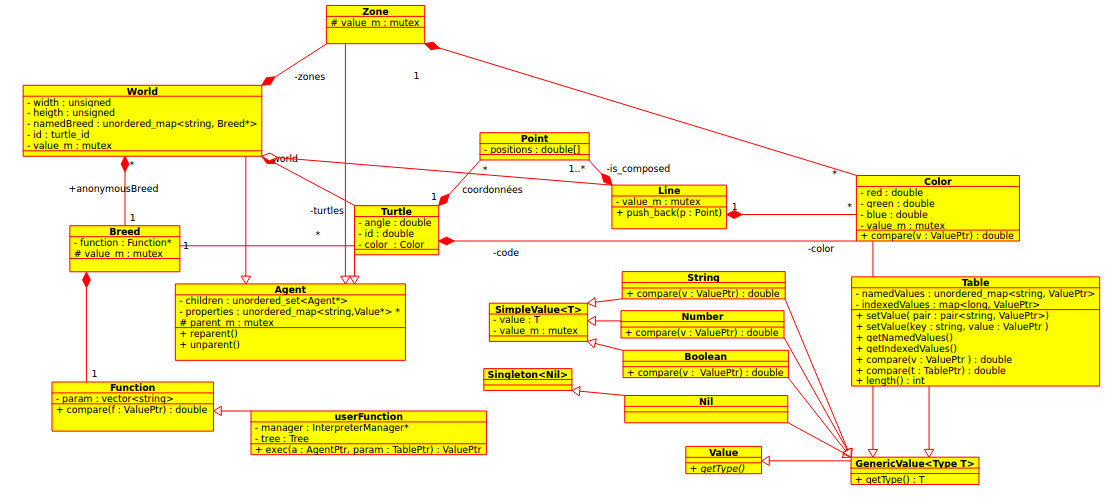
\includegraphics[scale=0.4]{doc/report/uml/v03.png}
\caption{\label{v0.3} UML version 0.3}
\end{figure}

Nous avons mis en place des mutex récursifs lors du quatrième sprint. Ils permettent à un thread de verrouiller plusieurs fois la même ressource qu'il a déjà verrouillée. C'est la seule différence avec le mutex normal. 

Ces mutex permettent d'éviter des blocages dans certaines situations (fonctions récursives, etc.).
L'UML \ref{v0.4} est l'état final du modèle, le sprint 5 n'y ayant apporté aucune modification.
\begin{figure}[h]
\centering
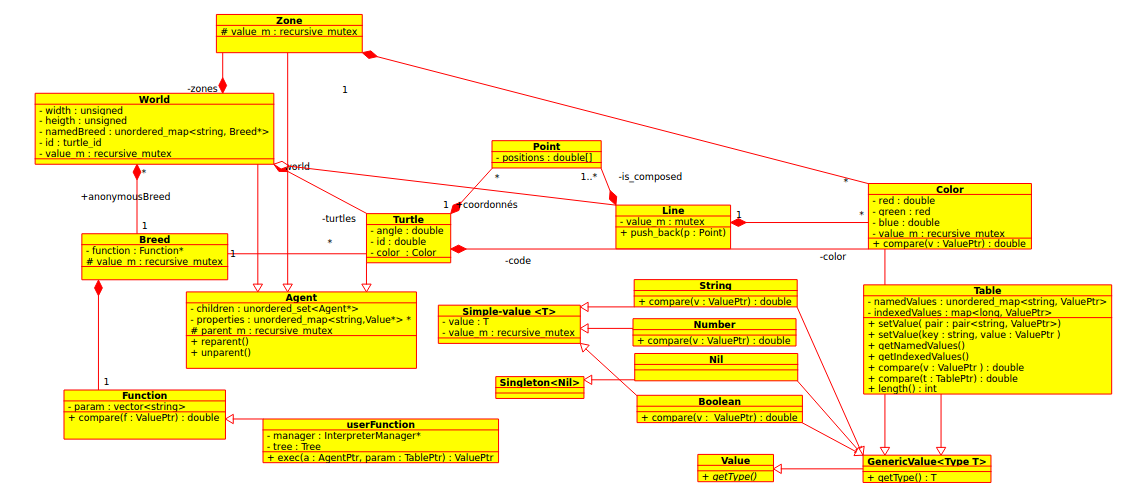
\includegraphics[scale=0.55, angle=90]{doc/report/uml/v04.png}
\caption{\label{v0.4} UML version 0.4}
\end{figure}

